\chapter{\iflanguage{ngerman}{Netzwerkkommunikation und Datenaustausch}{Network communication}}
\label{sec:overview}

Ein digitaler Datenbus der alle wichtigen Daten in Echtzeit zu Verfügung stellt und ermöglicht die medizinischen Geräte im OP-Saal über einen zentralen und übersichtlichen Zugriffspunkt zu steuern, ist im Moment noch nicht zur Realität geworden.\\
Die Netzwerkkommunikation und der Datenaustausch zwischen den medizinischen Geräten im OP-Saal werden durch herstellerabhängige Schnittstellen stark eingeschränkt. Bei der Installation eines Hybriden OP-Saals, muss ich derzeit für einen Hersteller entschieden werden, denn \glqq eine Integration von Drittanbieterkomponenten kann nur in Kooperation mit dem Hersteller des Integrationssystems erfolgen\grqq{} \cite{DerDigitaleOperationssaal}.

Um diesen Problem entgegen zu wirken, wurde für eine herstellerübergreifende Netzwerkkommunikation die Service Oriented Architecture für den medizinischen Gebrauch angepasst und zum ungehinderten Datenaustausch Standards wie DICOM, HL7 und IHE entwickelt.

\subsection{Service Oriented Architecture}

\begin{figure} [H]
	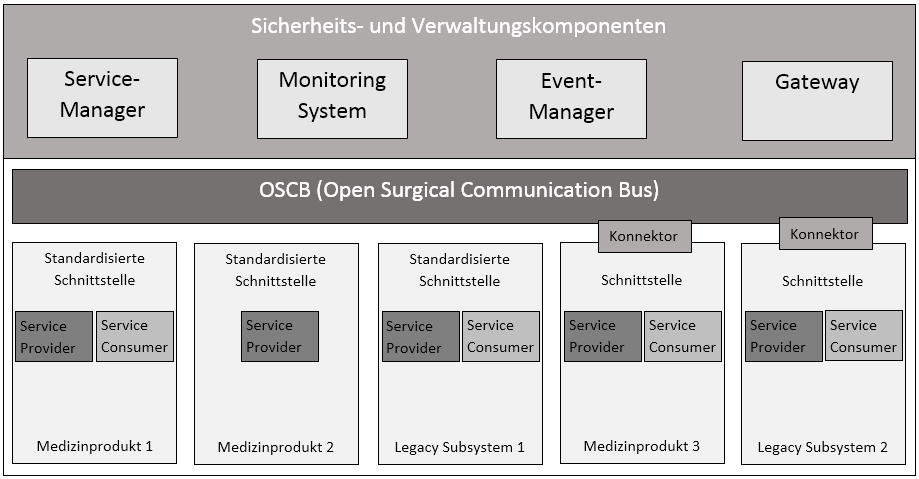
\includegraphics[scale = 0.6]{Content/Pictures/soa-red.png}
	\caption{SOA für den medizinischen Gebrauch im Operationssaal nach Abbild \cite{DerDigitaleOperationssaal}.}
	\label{fig:soa}
\end{figure}

In der Service Oriented Architecture (SOA, Abb. \ref{fig:soa}) für den medizinischen Gebrauch, interagieren Service Provider und Service Consumer über einen Open Surgical Communication Bus (OSCB). Dabei können die medizinischen Geräte sowohl Service Provider als auch Consumer sein und Dienste über eine standardisierte Schnittstelle nutzen bzw. bereitstellen. Der Service Manager verwaltet alle verfügbaren Geräte und Dienste im Netzwerk. Service Consumer können dann über den Service Manager Dienste und Geräte anfragen, welcher dann verfügbare und passende Service Provider zurück gibt. Nach diesem Schritt läuft die Kommunikation direkt zwischen Consumer und Provider ab. 
Die Übertragung von Daten und die Kommunikation zwischen den medizinischen Geräten läuft also immer über den OSCB ab. Um eine reibungslose Vernetzung zu ermöglichen sind standardisierte herstellerübergreifende Schnittstellen essentiell.  
Für Geräte die kein standardisiertes Datenformat (wie DICOM) zu Verfügung stellen, übernimmt ein Konnektor die Aufgabe der Transformation und ermöglicht eine höhere Bandbreite an Geräten die verwendet werden können. Kommunikation die über den Operationssaal hinaus mit anderen Netzwerken der Klinik statt findet, wird immer über eine Gateway geleitet, um eine höhere Sicherheit zu gewährleisten.
Weitere optionale Komponenten in der SOA sind der Event Manager, welcher auftretende Ereignisse verwaltet und gegebenenfalls andere Geräte im Netzwerk darüber informiert und das Monitoring System, welches zur Unterstützung des Service Managers eingesetzt wird, zur Überwachung alle angeschlossenen Geräte, um fehlerhafte Services zu identifizieren \cite{DerDigitaleOperationssaal}. 

Webservices bieten durch ihre lose Client Server Kopplung und einfache Erweiterbarkeit eine gute Möglichkeit, um SOA im medizinischen Umfeld einzusetzen. Zur Verwirklichung des OSCBs bietet Ethernet aufgrund der hohen Bandbreite und der bereits bestehenden Infrastruktur in Krankenhäusern eine gute Grundlage für die Vernetzung. Gleichzeitig ist aber die Gewährung der Sicherheit und Zuverlässigkeit des Systems mit einem höheren Aufwand verbunden als bei anderen Technologien.
Die tatsächliche Client Server Kommunikation wird dann je nach Anwendungsfall mit TCP oder UPD verwirklicht \cite{DerDigitaleOperationssaal}.

Dieser Ansatz der Umsetzung einer SOA im medizinischen Umfeld, ermöglicht alle Geräte im Netzwerk über eine zentrale Anzeige im Operationssaal zu kontrollieren. Dazu gehören nicht nur die bildgebenden Verfahren, sondern auch der OP-Tisch, die Beleuchtungsanlagen und Kameras mit der Anzeigeausgabe auf den Monitoren \cite{DerDigitaleOperationssaal}.

OR.NET (Secure Dynamic Networking in Surgery and Clinic) ist ein Projekt welches auf der SOA basiert und die Integration von medizinischen Geräten und IT-Systemen demonstriert. Ziel ist es, die Gerätekommunikation im OP zu erleichtern, Echtzeitkommunikation möglich zu machen und eine internationale Normung für alle Operationssäle festzulegen. 
Zur Umsetzung dieses Projekts wurde ein neuer Substandard entwickelt. Dieser soll jedoch nicht bereits vorhandene Standards wie HL7 oder DICOM ersetzen, sondern Geräte und Systeme in das IT-Netzwerk einbinden, welche die genannten Standards nicht umsetzen können.
Zur Demonstration der Funktionsweise und Umsetzbarkeit von OR.NET wurden komplett funktionsfähige Operationssäle zusammengestellt (Abb. \ref{fig:ornet}), die alle benötigten medizinische Geräte und klinische IT-Systeme von unterschiedlichen Herstellern vereinen \cite{ORnet}.
Damit konnte gezeigt werden, dass eine einheitliche Mensch Maschine Interaktion unabhängig vom Gerät möglich ist. Durch die Vernetzung aller Daten kann problemlos während einer Operation auf präoperativ angefertigte Bilddateien, Patienteninformationen und Laborbefunde zugegriffen werden. Auch von außerhalb des Operationssaals kann der Oberarzt alle wichtigen Informationen einsehen, die im OP erfasst und aufgezeichnet werden. Neue Funktionalitäten, wie eine Datenbrille über die der Chirurg direkt Blutdruck und Herzfrequenz des Patienten übermittelt bekommt ohne seinen Blick abwenden zu müssen, können problemlos in das vernetzte System integriert werden. Alle chirurgischen Geräte können direkt angesteuert und teilweise auch mit Fußschaltern vom Chirurgen bedient werden. Damit wird die Abhängigkeit des Chirurgen vom Assistenten verringert \cite{ORnetWebsite}.

\begin{figure} [H]
	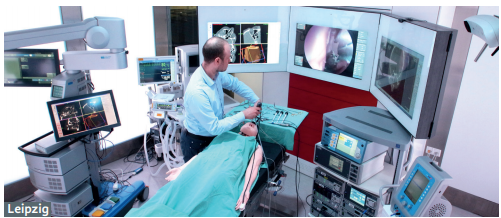
\includegraphics[scale = 0.8]{Content/Pictures/ornet.png}
	\caption{Operationssaal zur Demonstration von OR.NET in Leipzig, der in erster Linie für die Kopf- und Halschirurgie ausgelegt wurde \cite{ORnetWebsite}.}
	\label{fig:ornet}
\end{figure}

\subsection{Medizinische Standards}

Zur Kompatibilität medizinischer Geräte und Systeme unterschiedlicher Hersteller müssen gewisse Standards definiert werden.

Einer der am Weitesten verbreiteten Standards ist DICOM (Digital Imaging and COmmunications in Medicine). DICOM ist ein schnittstellenkompatibles Datenformat für die digitale medizinische Bildgebung. Es fungiert dabei nicht nur als Bildformat, sondern wird auch zum senden, verteilen und speichern medizinischer Bilder verwendet die von den bildgebenden Geräten (wie CT, MRT, US,..) erzeugt werden. Dabei ist das Ergebnis unabhängig vom Aufnahmegerät und Hersteller. DICOM ist auch für die richtige Darstellung der Bilder verantwortlich und ermöglicht nachträgliche Bildverarbeitung.
Zusätzlich bietet dieser Standard weitere Vorteile für die Dokumentation und Anzeige von medizinischen Bildern. So werden beispielsweise bis zu 65.536 (16 Bit) Grauschattierungen unterstützt, wobei im Gegensatz dazu bei einem JPG nur 256 verschiedene Grautöne möglich sind. Das verhilft selbst kleinste Details im aufgenommenen Bild richtig darzustellen und für den Chirurg erkenntlich zu machen. Zusätzlich werden zu jedem aufgenommenem Bild alle Daten, wie die Patienteninformationen oder Position des bildgebenden Geräts bei der Aufnahme, gespeichert \cite{DICOM}.

Ein weiterer Standard ist HL7 (Health Level Seven). HL7 ist ein schnittstellenkompatibler Kommunikationsstandard wie DICOM \cite{DerDigitaleOperationssaal} und bietet Protokolle für den Austausch, die Integration, Abfrage und Organisation von digitalen Gesundheitsinformationen die keine Bilddaten sind. Dabei wird festgelegt, mit welcher Sprache, Struktur und Datentypen Informationen in Pakete verpackt und versendet werden \cite{HL7}.

PACS (Picture Archiving Communication System) ist zur Darstellung, Analyse, Manipulation und zur Langzeit Archivierung aller erworbenen Bild- und Patientendaten. Direkt nachdem die Daten von einem Gerät erfasst wurden stehen sie zur Verfügung und können von mehreren Zugriffspunkten eingesehen werden \cite{PACS}.
So werden beispielsweise die Bilder im DICOM Format über das DICOM Netzwerk übertragen und dann von PACS als DICOM Objekte archiviert \cite{DICOM}.

Die genannten Standards weisen jedoch auch gewisse Limitierungen auf, aus welchem Grund IHE (Integrating the Healthcare Enterprise) entwickelt wurde. Dabei baut es auf Standards wie DICOM und HL7 auf und soll das Zusammenwirken sowie die Kommunikation unterschiedlicher IT-Systeme im medizinischen Umfeld verbessern \cite{DICOMundIHE}. 
IHE ist eine Initiative von Gesundheitsexperten einen weiteren Kommunikationsstandard zu entwickeln, um die Art und Weise zu verbessern, wie Computersysteme miteinander interagieren und Informationen austauschen. Mit IHE wird die Kommunikation zwischen unterschiedlichen Systemen verbessert, ist einfacher zu implementieren und ermöglicht Informationen effektiver zu nutzen \cite{IHE}.

Damit kann die Kompatibilität herstellerübergreifender Geräte und Systeme realisiert werden was zu einer höheren Flexibilität und verbesserten Möglichkeiten im Operationssaal führt \cite{DerDigitaleOperationssaal}.

\subsection{Sicherheitsprobleme und Datenschutz}

Mit der Digitalisierung und damit verbundenen Vernetzung der Geräte und Systeme im Operationssaal, spielt auch die Gewährleistung der Sicherheit und des Datenschutzes eine immer wichtigere Rolle.
Durch die enge Einbindung der medizinischen Geräte in das Netzwerk sind diese vermehrt Gefahren ausgesetzt und es müssen Schutzmaßnahmen ergriffen werden. Wie bereits in der Service Oriented Architecture erläutert, findet jegliche Kommunikation über den Operationssaal hinaus über ein Gateway statt. Eine Firewall wird eingesetzt, um den Datenverkehr zwischen dem OP- und Klinik-Netzwerk zu überwachen und gegebenenfalls Angriffe von außerhalb abzuwehren. Das alleine ist jedoch noch nicht ausreichend, sondern es muss zusätzlich auch sichergestellt werden, dass \glqq ein Medizingerät nur authentisierte, verifizierte und validierte Befehle entgegennimmt und ausführt\grqq{} \cite{DerDigitaleOperationssaal}. \\
Besonders im Bezug auf den Datenschutz ist eine \glqq vertrauliche Übermittlung von sensiblen Daten wie Patientenidentität, Vitalparameter, Krankengeschichte und Medikation unerlässlich\grqq{} \cite{DerDigitaleOperationssaal}, weshalb die Geräte und Daten vor unerlaubten Lese- und Schreibzugriffen geschützt werden müssen. Aus diesem Grunde müssen zur Sicherstellung von Integrität und Vertraulichkeit Nachrichten signiert und verschlüsselt werden \cite{DerDigitaleOperationssaal}. 

Wenn man beispielsweise Zugriff auf eine DICOM Datei hat, dann kann man selbst mit einem primitiven Editor wie Notepad ganz einfach sensible Daten wie den Patientennamen, behandelnden Arzt und das Krankenhaus herauslesen und verändern (Abb. \ref{fig:dicom}). Selbst das DICOM Bild kann mit geringen Programmierkenntnissen oder mit passender verfügbarer Software betrachtet, bearbeitet oder einfach ausgetauscht werden.\\
Aus diesem Grund müssen das Netzwerk und die versendeten Daten vor unberechtigtem Zugriff und Manipulation geschützt und gegebenenfalls anonymisiert werden. Konkret heißt das, dass jegliche Kommunikation über VPN läuft, die übertragenen Daten verschlüsselt und vor dem Lesen das Zugriffsrecht und Sender validiert werden und jeder Computer im Netzwerk durch eine Firewall geschützt wird \cite{DICOM}. 

Datenschutz muss in allen Bereichen der digitalen Medizintechnik gewährleistet und sichergestellt werden. Übergreifend ist damit nicht nur PACS und DICOM bzw. ersatzweise HL7 betroffen, sondern auch Radiologische Informationssysteme (RIS) und Krankenhaus Informationssysteme (HIS) \cite{DICOM}. 

\begin{figure} [H]
	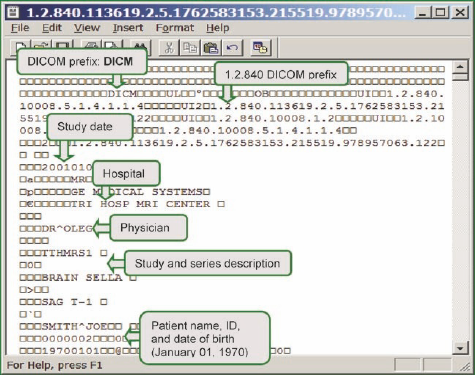
\includegraphics[scale = 0.7]{Content/Pictures/DICOMEditor.png}
	\caption{DICOM Datei in WordPad, aus der Patienteninformationen, Krankenhaus und behandelnder Arzt direkt ausgelesen werden können \cite{DICOM}}
	\label{fig:dicom}
\end{figure}
